\section{How to Apply for Data Center Tax Incentives}

\subsection{Texas}

Applicants must submit Form AP-233 or AP-236 to the Texas Comptroller of Public Accounts to register as a qualifying data center or qualifying large data center project and obtain a unique registration number. They must then provide the seller with an exemption certificate (Form 01-929) to claim the exemption.

The application must be accompanied by a capital investment plan, a job-creation plan, and a site plan or building schematic.

\begin{figure}[htbp]
\centering
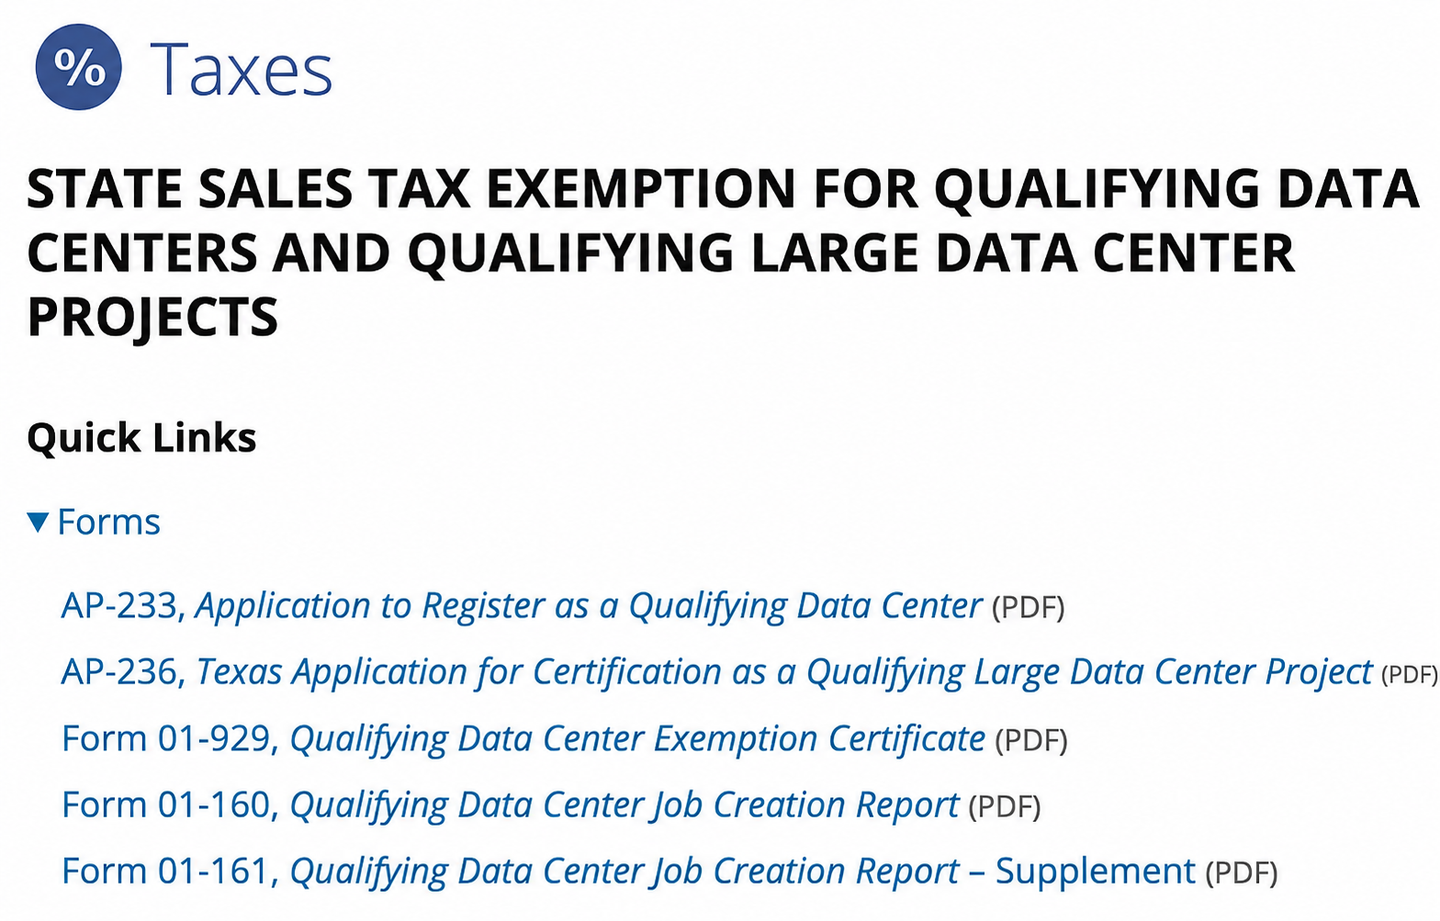
\includegraphics[width=0.48\linewidth,height=0.34\textheight,keepaspectratio]{assets/figure-5.png}\hfill
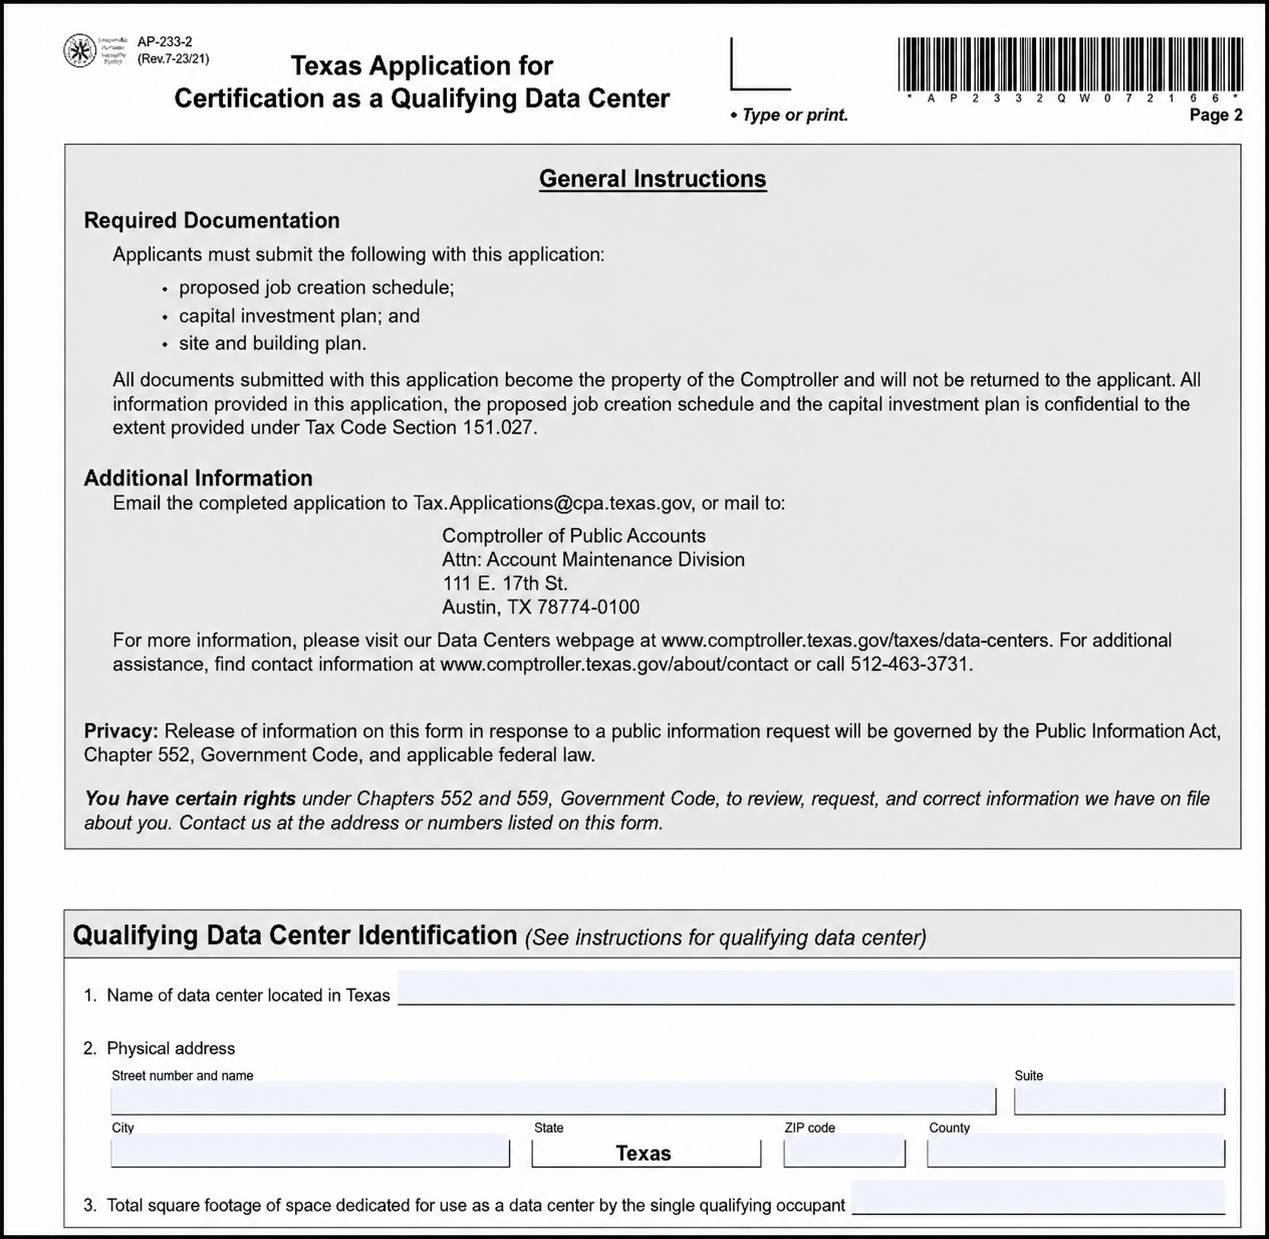
\includegraphics[width=0.48\linewidth,height=0.34\textheight,keepaspectratio]{assets/figure-6.png}
\caption{Texas Qualifying Data Center Application Forms Download Page (original Figures 2 and 3).}
\end{figure}

Application forms:

\url{https://comptroller.texas.gov/taxes/data-centers}

\FloatBarrier
\subsection{Virginia}

To apply for the DCRSUT Exemption, a qualifying data center must negotiate and execute a Memorandum of Understanding (MOU) with the Virginia Economic Development Partnership (VEDP). VEDP submits the MOU to the Virginia Department of Taxation for review; once approved, the Department of Taxation issues an Exemption Certificate directly to the data center.

A tenant of a colocation data center must separately enter into a Participation Certificate and Agreement with the data center. After VEDP and the Virginia Department of Taxation review the Participation Certificate and Agreement, the Department of Taxation issues a separate Exemption Certificate directly to the tenant.

MOU download:

\url{https://www.vedp.org/incentive/data-center-retail-sales-use-tax-exemption}

\subsection{Georgia}

A Data Center Owner or High-Technology Data Center Customer may submit an application for a certificate of exemption through the Georgia Tax Center (GTC). The Department will not issue a certificate of exemption to a customer until a certificate of exemption has been issued to the corresponding Data Center Owner.

As part of the application, a data center may be required to provide the applicant's Georgia income tax filing and payment history, the value of the applicant's title or interest in Real Property owned in the state, documentation sufficient to demonstrate the likelihood of satisfying the High-Technology Data Center Minimum Investment Threshold, and other supporting materials. A High-Technology Data Center Customer may be required to submit a copy of its data center services contract, among other documents.

Application instructions:

\url{https://dor.georgia.gov/how-apply-high-technology-data-center-exemption}

\FloatBarrier
